\documentclass[12pt,a4paper]{article}
\usepackage{cmap} % Makes the PDF copiable. See http://tex.stackexchange.com/a/64198/25761
\usepackage[T1]{fontenc}
\usepackage[brazil]{babel}
\usepackage[utf8]{inputenc}
\usepackage{amsmath}
\usepackage{amsfonts}
\usepackage{amssymb}
\usepackage{amsthm}
\usepackage{textcomp} % \degree
\usepackage{gensymb} % \degree
\usepackage[usenames,svgnames,dvipsnames]{xcolor}
\usepackage{hyperref}
\usepackage{multicol}
\usepackage{graphicx}
\usepackage[margin=2cm]{geometry}
\usepackage{systeme}

\hypersetup{
    colorlinks = true,
    allcolors = {blue}
}

% TODO: Consider using exsheets
% http://linorg.usp.br/CTAN/macros/latex/contrib/exsheets/exsheets_en.pdf
%
% http://ctan.org/tex-archive/macros/latex/contrib/exercise/
% Options: answerdelayed,lastexercise,noanswer
\usepackage[answerdelayed,lastexercise]{exercise}

\addto\captionsbrazil{%
\def\listexercisename{Lista de exerc\'icios}%
\def\ExerciseName{Exerc\'icio}%
\def\AnswerName{Solu\c{c}\~ao do exerc\'icio}%
\def\ExerciseListName{Ex.}%
\def\AnswerListName{Solu\c{c}\~ao}%
\def\ExePartName{Parte}%
\def\ArticleOf{de\ }%
}

\renewcommand{\ExerciseHeaderTitle}{(\ExerciseTitle)\ }
\renewcommand{\ExerciseListHeader}{%\ExerciseHeaderDifficulty%
\textbf{%\ExerciseListName\
\ExerciseHeaderNB.\ %
%\ --- \
\ExerciseHeaderTitle}%
%\ExerciseHeaderOrigin
\ignorespaces}
\renewcommand{\AnswerListHeader}{\textbf{\ExerciseHeaderNB.\ (\AnswerListName)\ }}

\newcommand{\fixme}{{\color{red}(...)}}
\newcommand*\R{\mathbb{R}}

% Loop Space / CC BY-SA-3.0 / https://tex.stackexchange.com/a/2238/25761
\newenvironment{amatrix}[1]{%
  \left[\begin{array}{@{}*{#1}{c}|c@{}}
}{%
  \end{array}\right]
}

% Loop Space / CC BY-SA-3.0 / https://tex.stackexchange.com/a/3164/25761
%--------grstep
% For denoting a Gauss' reduction step.
% Use as: \grstep{\rho_1+\rho_3} or \grstep[2\rho_5 \\ 3\rho_6]{\rho_1+\rho_3}
\newcommand{\grstep}[2][\relax]{%
   \ensuremath{\mathrel{
       {\mathop{\longrightarrow}\limits^{#2\mathstrut}_{
                                     \begin{subarray}{l} #1 \end{subarray}}}}}}

\renewcommand{\theenumi}{\alph{enumi}}
\renewcommand\labelenumi{(\theenumi) }

\newcommand*\tipo{Prova IV}
\newcommand*\turma{PRO112-02U}
\newcommand*\disciplina{ALI0001}
\newcommand*\eu{Helder G. G. de Lima}
\newcommand*\data{06/12/2017}

\author{\eu}
\title{\tipo - \disciplina}
\date{\data}

\begin{document}
\thispagestyle{empty}
\newgeometry{margin=2cm,bottom=0.5cm}
\begin{center}

\includegraphics[width=9.0cm]{marca} \\
\textbf{\tipo\ (\disciplina / \turma)} \\
Prof. \eu\footnote{
Este é um material de acesso livre distribuído sob os termos da licença \href{https://creativecommons.org/licenses/by-sa/4.0/deed.pt_BR}{Creative Commons BY-SA 4.0}}
\end{center}

\noindent Nome do(a) aluno(a): \underline{\hspace{9,7cm}} Data: \underline{\data}

%\section*{Instruções}
\begin{center}\fbox{
\begin{minipage}{14cm}

{\footnotesize
\begin{itemize}
\renewcommand{\theenumi}{\Roman{enumi}}
\item Identifique-se em todas as folhas.
\item Mantenha o celular e os demais equipamentos eletrônicos desligados durante a prova.
\item Resolva (integralmente) apenas os itens de que precisar para somar 10,0 pontos.
\end{itemize}
}

\end{minipage}
}
\end{center}

\section*{Questões}
\begin{ExerciseList}
\Exercise[title={1,0}] Explique o que é um autovetor e um autovalor e interprete geometricamente.
\Answer \fixme

\Exercise[title={3,0}] Suponha que um operador linear $T: \R^2 \to \R^2$ transforma os pontos indicados na \autoref{fig:dom} nos pontos correspondentes da \autoref{fig:cd}:
\begin{figure}[h]
    \centering
    \begin{minipage}{0.45\textwidth}
        \centering
        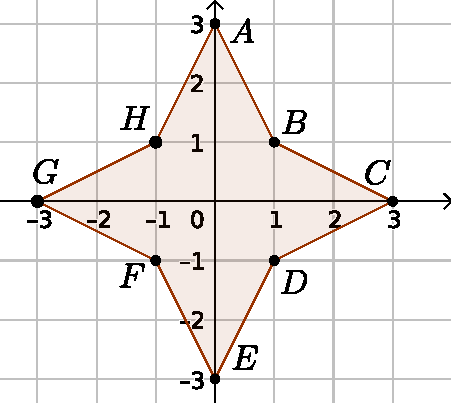
\includegraphics[height=0.48\textwidth]{img/prova-4-pro-dom}
        \caption{Domínio}\label{fig:dom}
    \end{minipage}\hfill
    \begin{minipage}{0.45\textwidth}
        \centering
        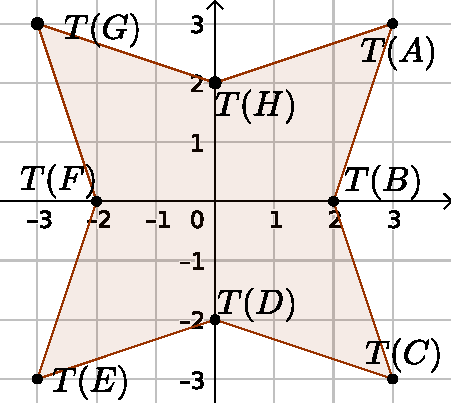
\includegraphics[height=0.48\textwidth]{img/prova-4-pro-img}
        \caption{Contradomínio}\label{fig:cd}
    \end{minipage}
\end{figure}
\begin{enumerate}
\item Qual é a fórmula para $T(x,y)$?
\item O que se pode afirmar sobre os autovalores e os autovetores de $T$? Justifique sua resposta.
\end{enumerate}
\Answer \fixme

\Exercise[title={3,0}] Classifique cada afirmação como \textbf{verdadeira} ou \textbf{falsa}, justificando sua resposta:
\begin{enumerate}
\item O operador identidade $T: \R^3 \to \R^3$, dado por $T(v) = v, \forall v \in \R^3$, é diagonalizável.
\item Se $\lambda = 0$ é um autovalor de um operador $T : V \to V$ então $T$ não é um isomorfismo.
\item Existem matrizes semelhantes $A$ e $B$ tais que $\det(A) \neq \det(B)$.
\end{enumerate}
\Answer \fixme

\Exercise[title={3,0}] Seja $A =
\begin{bmatrix}
2 & 1 \\ 0 & 3
\end{bmatrix}$.
\begin{enumerate}
\item Obtenha, se possível, uma matriz $P$ e uma matriz diagonal $D$ tais que $A = P D P^{-1}$.
\item Utilize o item anterior para calcular a matriz $M = A^5$.
\end{enumerate}
\Answer \fixme

\Exercise[title={3,0}] Seja $T : \R^3 \to \R^3$ o operador linear definido por
\[
T(x,y,z) = (3x-2y+z, -y, -12x+6y-4z).
\]
Verifique se $T$ é diagonalizável, e justifique sua resposta.
\Answer \fixme
\end{ExerciseList}

\begin{center}
BOA PROVA E BOAS FÉRIAS!
\end{center}

%\newpage
%\restoregeometry
%\section*{Respostas}
%\shipoutAnswer
\end{document}
